
-- How likely is the symmetry assumption in cortical circuits? --

However, even when pairs . This can be demonstrated by considering a model of in which .

Consider for this that connection probabilities $P_{ij}$ are distributed according to some probability density function $f_{P_{ij}}$. We assume in the following that $i > j$ without restriction. The expected probability of a reciprocal connection within a pair can be expressed as
%
\begin{align}
  \E(P_{ij}P_{ji}) = \int_0^1 \int_0^1 xy\, f_{P_{ij},P_{ji}}(x,y) \, dx\, dy, \label{eq:dbint}
\end{align}
%
where $f_{P_{ij},P_{ji}}(x,y)$ is the joint probability density function of $P_{ij}$ and $P_{ji}$, 
%
\begin{align}
  f_{P_{ij},P_{ji}}(x,y) =  f_{P_{ji} | P_{ij}}(y \mid x) f_{P_{ij}}(x). \label{eq:cdf_def}
\end{align}
%
In the case that $P_{ij}$ and $P_{ji}$ are independent we have $f_{P_{ji} | P_{ij}}(y \mid x) = f_{P_{ji}}(y)$ and in the case of $P_{ij}=P_{ji}$ it is $f_{P_{ji} | P_{ij}}(y \mid x) = \delta(y-x)$. Here we propose a model for the conditional density function that transitions between the two extreme cases by multiplying $f_{P_{ji}}(y)$ with the density function of a normal distribution centered around $x$,
%
\begin{align}
  f_{P_{ji} | P_{ij}} (y \mid x) = \frac{1}{N_{\sigma}(x)} f_{P_{ji}}(y)\, \frac{1}{\sigma \sqrt{2 \pi}} \,e^{\frac{(y-x)^2}{2 \sigma^2}} \label{eq:fpijpji},
\end{align}
%
where the additional factor $N_{\sigma}(x)^{-1}$  makes sure that $f_{P_{ji}|P_{ij}} (y \mid x)$ integrates to one,
%
\begin{align}
  N_{\sigma}(x) = \int_0^1 f_{P_{ji}}(z)\, \frac{1}{\sigma \sqrt{2 \pi}}\, e^{\frac{(z-x)^2}{2 \sigma^2}} \,dz.
\end{align}
%
Indeed, as the standard deviation $\sigma$ of the modulating normal distribution increases $f_{P_{ji}|P_{ij}} (y \mid x) \to f_{P_{ji}}(y)$ and in the limit $\sigma \to 0$ we have
\begin{align}
  \lim_{\sigma \to 0}   f_{P_{ji}|P_{ij}} (y \mid x) = \delta(y-x).
\end{align}
%
In Figure~\ref{fig:sym_fail}A  conditional density functions for various $\sigma$ are shown for the truncated gamma distribution. For low values of $\sigma$ the conditional density function resembles a narrow Gaussian around $x$, reflecting approximately symmetric connection probabilities. For $\sigma > 1$ on the other hand $f_{P_{ji} | P_{ij}}(y \mid x)$ becomes virtually indistinguishable from $f^T_{\alpha, \beta}(y)$, signifying independence of $P_{ji}$ from $P_{ij}$.

Finally we employ the model to examine how the relative overrepresentation of bidirectional connections $\varrho$ changes with the degree of symmetry in the connection probabilities within a pair of neurons. For this $\varrho$ is computed as a function of $\sigma$ as for a given distribution of $P_{ij}$ as
%
\begin{align}
  \varrho = \frac{\E(P_{ij} P_{ji})}{\mu^2}, \label{eq:rho_sigma}
\end{align}
%
where the numerator is given by \eqref{eq:dbint} with %\eqref{eq:cdf_def} and
\eqref{eq:fpijpji} %,
%
%% \begin{align}
%%   \E(P_{ij}P_{ji}) = \int_0^1 \int_0^1 xy\, f_{P_{ij}}(x) \frac{1}{N_{\sigma}(x)} f_{P_{ji}}(y)\, \frac{1}{\sigma \sqrt{2 \pi}} \,e^{\frac{(y-x)^2}{2 \sigma^2}} \, dx\, dy,  
%% \end{align}
%
and the overall connection probability $\mu$ is calculated as
%
\begin{align}
 \mu = \frac{1}{2} \int_0^1 x f_{P_{ij}}(x)\,dx + \frac{1}{2} \int_0^1 f_{P_{ij}}(x) \int_0^1 y \,f_{P_{ji}\vert P_{ij}}(y \mid x) \,dy \, dx.
\end{align}
%

Figure~\ref{fig:sym_fail}B shows the change of $\varrho$ with $\sigma$ for connection probabilities $P_{ij}$ following a truncated gamma distribution $\Gamma^T(\alpha, \beta)$. For the three parameters sets chosen, we can show that a strong overrepresentation of bidirectional connections . In fact as along 

\begin{figure}[h!]
\centering
%% \begin{overpic}[width=0.495\textwidth]%
%%   {../../../lab/bench/fig3A/fig3A.pdf}
%%   \put(18.,66.5){\textbf{A}}
%% \end{overpic}
%% \begin{overpic}[width=0.495\textwidth]%
%%   {../../../lab/bench/fig3B/fig3B.pdf}
%%   \put(18.,66.5){\textbf{A}}
%% \end{overpic}
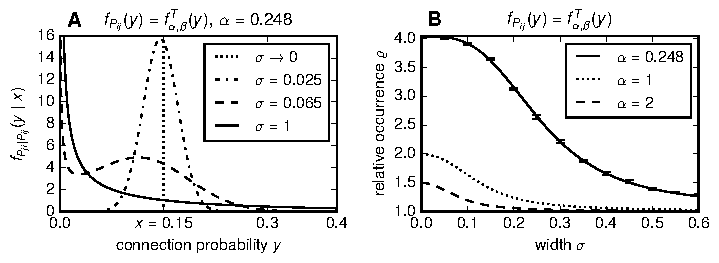
\includegraphics[width=\textwidth]{%
  /home/fh/sci/rsc/nrnd_pairs/pub/arxiv_16/figures/sym_fail/sym_fail_figure.png}
\caption{Relative overrepresentation of bidirectional connections $\varrho$ is sustained when connection probabilities are only approximately symmetric in pairs. \textbf{A} Illustration how the conditional density function $f_{P_{ji} | P_{ij}} (y\,\vert\, x)$ of \eqref{eq:fpijpji} transitions from equality of the random variables $P_{ij}$ and $P_{ji}$ to independence with increasing $\sigma$. It is $f_{P_{ij}} (y) = f^T_{\alpha,\beta}(y)$, with $\alpha=0.248$ and $\beta$ such that $\operatorname{E}(P_{ij})=0.1$. For the illustration $P_{ij}$ was fixed as $x=0.15$. Already for $\sigma=1$ the conditional density function becomes visually indistinguishable from  $f^T_{\alpha,\beta}(y)$ in the graphic. \textbf{B}~Relative occurrence of reciprocally connected pairs $\varrho$ as a function of $\sigma$. The curves for $\alpha=1$ and $\alpha=2$ show numerical solutions of \eqref{eq:rho_sigma} with $f_{P_{ij}} = f_{\alpha,\beta}^T$, where $\beta$ was chosen such that $\operatorname{E}(P_{ij}) = 0.1$. For $\alpha = 0.248$ random variables with the respective probability density functions were sampled and the average $\varrho$ was computed via \eqref{eq:rho_sigma} using the sample means. Error bars show SEM, the curve for $\alpha = 0.248$ (solid line)  was fitted to the data points and is purely for illustrative purposes.} 
\label{fig:sym_fail}
\end{figure}


%
%% and
%% %
%% \begin{align}
%%   \lim_{\sigma \to \infty}   f_{P_{ji}|P_{ij}} (y \mid x) = f_{P_{ji}}(y)
%% \end{align}
%% Expression $\eqref{eq:rho}$ can then be written as
%% %
%% \begin{align}
%% \varrho = \frac{\E(P_{ij}P_{ji})}{{\E\left(P_{ij}\right)}^2} = \frac{\int_0^1 \int_0^1 xy\, f_{P_{ij}P_{ji}}(x,y) \, dx\, dy}{\left(\int_0^1 x f_{P_{ij}}(x)\, dx\right)^2}
%% \end{align}

